\documentclass{beamer}
\usetheme[progressbar=frametitle]{metropolis}          % Use metropolis theme

% change progressbar thickness
\makeatletter
\setlength{\metropolis@titleseparator@linewidth}{1.5pt}
\setlength{\metropolis@progressonsectionpage@linewidth}{1.5pt}
\setlength{\metropolis@progressinheadfoot@linewidth}{2pt}
\makeatother

\usepackage{FiraSans}
\usepackage{makecell}
\usepackage{appendixnumberbeamer}

\title{Ovlivnění nazality poruchou basálních ganglií}
\date{9. 1. 2020}
\author{Vojtěch Illner \& Tomáš Hyhlík}
\institute{Semestrální projekt B2M31AEDA, 2019/20}
\begin{document}
  \maketitle

  \begin{frame}{Úvod}
    Výrazný aspekt neurodegenerativních onemocnění je dopad na motorické schopnosti.
    
    Mezi nejčastější patří Parkinsonova (PN) a Huntingtonova nemoc (HN).
    
    S tím spojený velice častý výskyt poruchy řeči.
    
    Zde zkoumána jedna z jejích charakteristik - \textbf{hypernazalita}.
    
  \end{frame}

  \begin{frame}{Hypernazalita}
	Jedná se o patologicky zvýšenou \emph{nosovost}.
	
	Různé příčiny u HN a PN.
	
	Může sloužit jako užitečný biomarker? 
	\begin{itemize}
		\item Trpí pacient neurodegenerativní chorobou? Popřípadě jakým typem?
		\item Dá se zjišťovat závažnost nemoci? 
	\end{itemize}
  \end{frame}

  \begin{frame}{Data}
  	\begin{alertblock}{Řečová data}
  		Úloha prodloužené fonace hlásky /i/ a krátký monolog.
  		
  		Pořízena od 37mi zdravých lidí (HC), 37mi pacientů s PN a 37mi s HN.
  		
  		Závažnost onemocnění hodnocena podle standardizovaných škál UPDRS III a UHDRS.
  	\end{alertblock}
    \begin{alertblock}{Akustické příznaky nazality}
    	Vypočítány z prodloužené fonace pomocí algoritmu analýzy třetino-oktávového spektra \cite{algorithm}.
    	\begin{columns}[T,onlytextwidth]
    		\column{0.33\textwidth}
    		Míra
    		\begin{itemize}
    			\item EFN mean
    		\end{itemize}
    		
    		\column{0.33\textwidth}
    		Kolísavost
    		\begin{itemize}
    			\item EFN SD
    		\end{itemize}
    		
    		\column{0.33\textwidth}
    		Nárůst v čase
    		\begin{itemize}
    			\item EFN trend
    		\end{itemize}
    	\end{columns}
    Subjektivní vyhodnocení nezávislými hodnotiteli z řečového monologu.
    \end{alertblock}
  \end{frame}

  \begin{frame}{Použité statistické testy}
  	Předpoklady
  	\begin{itemize}
  		\item Normalita dat: Shapiro-Wilcoxon test
  		\item Rovnost rozptylů: Bartlett test
  	\end{itemize}
    Skupinové rozdíly + vliv pohlaví na výsledky
    \begin{itemize}
    	\item two-way ANOVA
    	\item Post-hoc vyhodnocení pomocí Bonferroniho metody
    \end{itemize}
    Reflexe závažnosti onemocnění
    \begin{itemize}
    	\item Spearmanův korelační test
    	\item Holm-Bonferroniho korekce (kvůli chybám 2. druhu)
    \end{itemize}
  \end{frame}

  \begin{frame}{Výsledky}
  	Normalitu dat zamítáme pro všechny veličiny a rovnost rozptylů pro dvě, \emph{EFN SD} a \emph{EFN trend}, při hladině významnosti $ \alpha=0.05 $.
  	
  	
  	\begin{alertblock}{Two-way ANOVA}
  		\begin{table}[h]
  			\footnotesize
  			\begin{tabular}{l|c|c|c|c|}
  				\multicolumn{1}{r}{}& \multicolumn{1}{r}{EFN mean} & \multicolumn{1}{r}{EFN SD} & \multicolumn{1}{r}{EFN trend} & \multicolumn{1}{r}{mean rates} \\ \cline{2-5}
  				typ onemocnění & $ p< 0.001 $ & $ p< 0.001 $ & n. s. & $ p<0.001 $ \\ \cline{2-5}
  				pohlaví & n. s. & n. s. & n. s. & n. s. \\ \cline{2-5}
  				\makecell{typ onemocnění \\ $ \times $ \\ pohlaví} & n. s. & n. s. & n. s. & n. s. \\ \cline{2-5}
  			\end{tabular}
  		\end{table}
  	\end{alertblock}
  \end{frame}

  \begin{frame}{Výsledky}
  	Post-hoc testy:
  	\begin{figure}
  		\centering
  		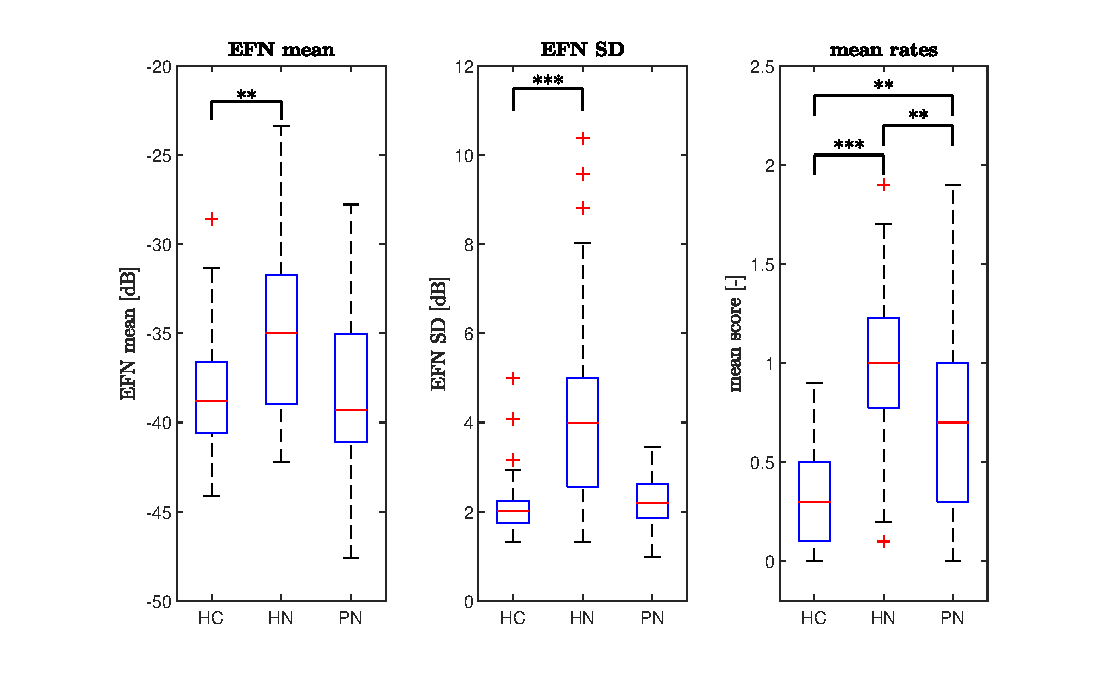
\includegraphics[width=0.7\linewidth]{boxplot.eps}
  	\end{figure}
  Spearmanův korelační test po přepočítání Holm-Bonf. korekcí nenalezl žádný signifikantní případ korelace ($ \alpha=0.05 $), až na dvě výjimky u HN. 	
  \end{frame}

  \begin{frame}{Interpretace}
  Typ onemocnění (HC, PN, HN) má zásadní vliv na měřené veličiny \emph{EFN mean} a \emph{EFN SD}, i na subjektivní skóre hodnotitelů.
  
  Nezajímavý parametr \emph{pohlaví} nemá žádný signifikantní vliv, stejně jako jeho interakce s typem nemoci.
  
  Naměřené veličiny \emph{EFN mean} a \emph{EFN SD} mají signifikantní rozdíly \emph{pouze} mezi skupinou HC a HN.
  
  Subjektivní hodnocení má významné rozdíly mezi \emph{všemi} skupinami.
  
  V naprosté většině případů nebyla nalezena signifikantní korelace mezi měřenou veličinou a hodnotami na stand. škále, což platilo i pro subjektivní hodnocení.
  \end{frame}

  \begin{frame}{Limitace práce}
  	Velké limitace a omezená věrohodnost především v předpokladech použitých testů (two-way ANOVA).
  	
  	Naštěstí bylo zjištěno, že ANOVA není tolik citlivá na rozumné odchylky od normálního rozdělení \cite{normalita}.
  	
  	Na zpřesnění výsledků by bylo možné použít složitější, více robustní neparametrické metody. 
  \end{frame}

  \begin{frame}{Závěr}
  	Veličiny \emph{EFN mean} a \emph{EFN SD} fungují jako účinné charakteristiky pro odlišení HC a HN. Pro PN skupinu nebyly zjištěny žádné významné rozdíly.
  	
  	\emph{EFN trend} nezaznamenal žádný signifikantní rozdíl mezi skupinami.
  	
  	Až na výjimky, naměřené veličiny nereflektují závažnost nemoci, danou stand. škálami.
  \end{frame}

  \begin{frame}{Budoucí práce}
  	V oblasti automatického vyhodnocování hypernazality mají dosavadní metody stále \emph{horší výsledky} než subjektivní hodnocení.

	V některých úlohách již ale stojí na podobné úrovni, např. při přítomnosti HN.
	
	 Automatické vyhodnocení pak přináší velké výhody při šetření času, 
	objektivitu a možnost detailních analýz, např. průběh nemoci, účinnost medikace.
  \end{frame}

  \appendix
  
  \begin{frame}{Reference}
  	
  	 \bibliography{aeda_prezentace_bib}
	 \bibliographystyle{abbrv}
  	
  \end{frame}

\end{document}